\chapter{Appendix for Aromaticity as a Guide to Planarity in Conjugated Molecules and Polymers}

\section{Different Length Polymer Chains}
\begin{figure}[hbt!]
    \centering
    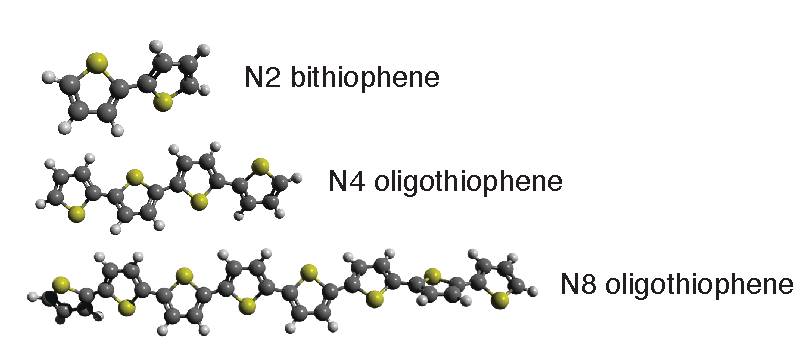
\includegraphics{figures/append_aroma/p_chains_graphic_copy.pdf}
    \caption{Different length oligomers of thiophene.}
    \label{fig:p_chains}
\end{figure}

\subsection{Comparison of Torsion Potentials}
\begin{figure}[hbt!]
    \centering
    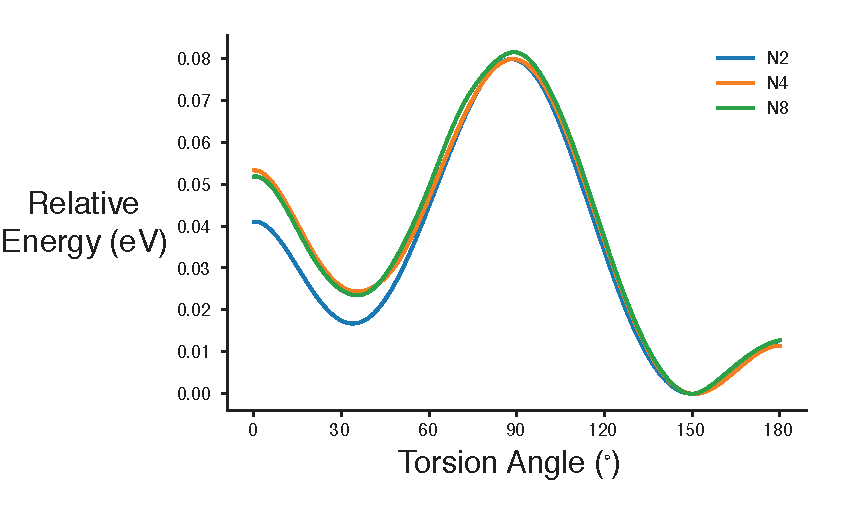
\includegraphics{figures/append_aroma/p_tor_compare_copy.pdf}
    \caption{The torsion potential of N2, N4, and N8 thiophene oligomers. All calculations were performed using the $\omega$B97x-D functional. The N2 torsion potential was calculated with the def2-TZVPP basis set, while N4 and N8 utilized the 6-31++G**\cite{Hehre1972} basis set to reduce to the computational cost. The deviation of N2 from both N4 and N8 between 0 and 50\textdegree \ is likely due to the different basis sets employed.}
    \label{fig:p_tor_compare}
\end{figure}

\clearpage
\subsection{Comparison of NICS Aromaticity}
\begin{figure}[hbt!]
    \centering
    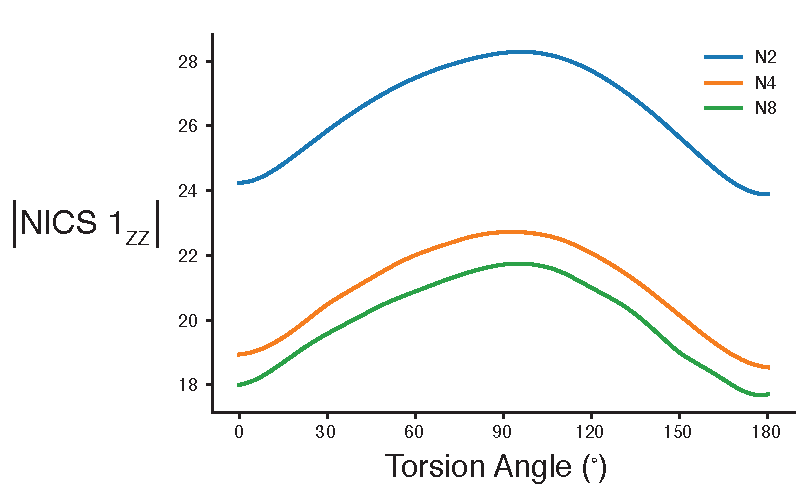
\includegraphics{figures/append_aroma/p_NICS_compare_copy.pdf}
    \caption{N2, N4, and N8 absolute NICS $1_{ZZ}$ values as a function of torsion angle. The magnitude of NICS values decrease with chain length, and we expected that the values will converge once a certain chain length is reached. While the magnitude decreases the overall trend as a function of torsion angle is consistent, which allows N2 to represent larger chains.}
    \label{fig:p_NICS_compare}
\end{figure}

\clearpage
\section{Comparision of MCI and NICS Aromaticity Values}

\subsection{BT}
\begin{figure}[hbt!]
    \centering
    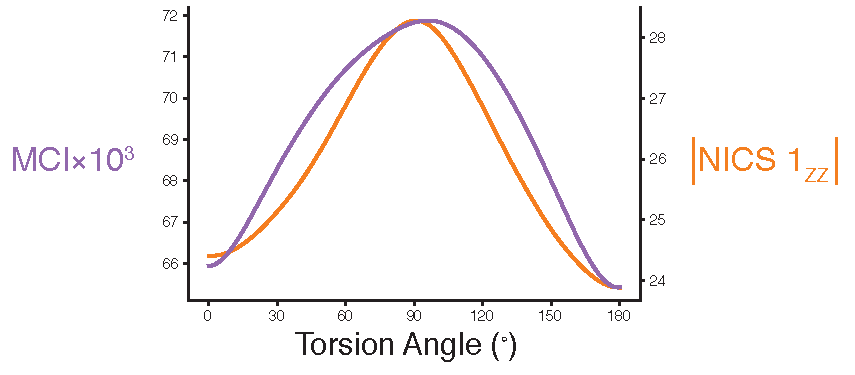
\includegraphics{figures/append_aroma/pt_aroma_compare_copy.pdf}
    \caption{Comparison of the aromaticity indexes MCI and NICS for BT.}
    \label{fig:pt_aroma_compare}
\end{figure}

\subsection{hBT}
\begin{figure}[hbt!]
    \centering
    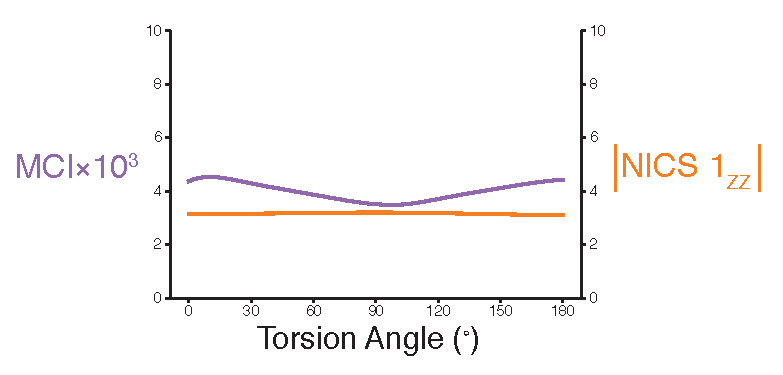
\includegraphics{figures/append_aroma/hpt_aroma_compare_copy.pdf}
    \caption{Comparison of the aromaticity indexes MCI and NICS for hBT.}
    \label{fig:hpt_aroma_compare}
\end{figure}

\clearpage
\subsection{F2-BT}
\begin{figure}[hbt!]
    \centering
    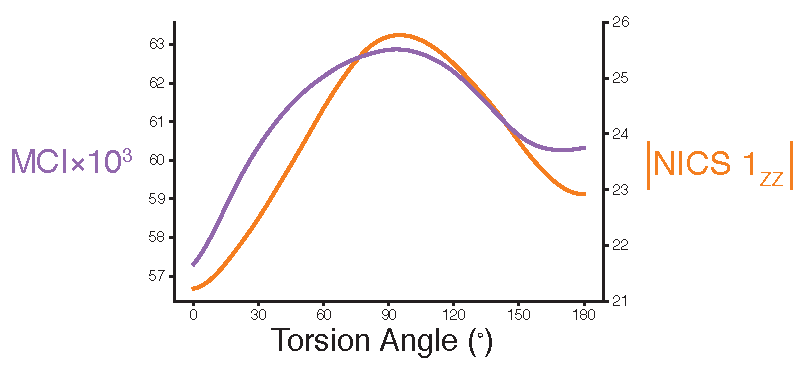
\includegraphics{figures/append_aroma/pt_f2_aroma_compare_copy.pdf}
    \caption{Comparison of the aromaticity indexes MCI and NICS for F2-BT.}
    \label{fig:pt_f2_aroma_compare}
\end{figure}


\subsection{BEDOT}
\begin{figure}[hbt!]
    \centering
    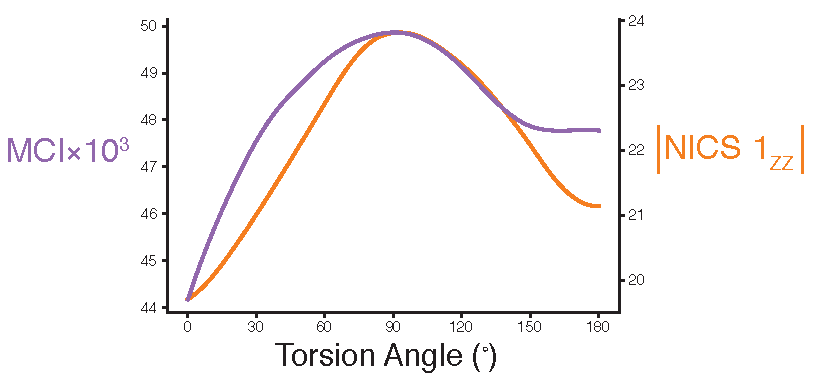
\includegraphics{figures/append_aroma/pedot_aroma_compare_copy.pdf}
    \caption{Comparison of the aromaticity indexes MCI and NICS for BEDOT.}
    \label{fig:pedot_aroma_compare}
\end{figure}

\clearpage
\section{Through-space Calculations}
\subsection{\texorpdfstring{H $\cdots$ S}{HS}}
\begin{figure}[hbt!]
    \centering
    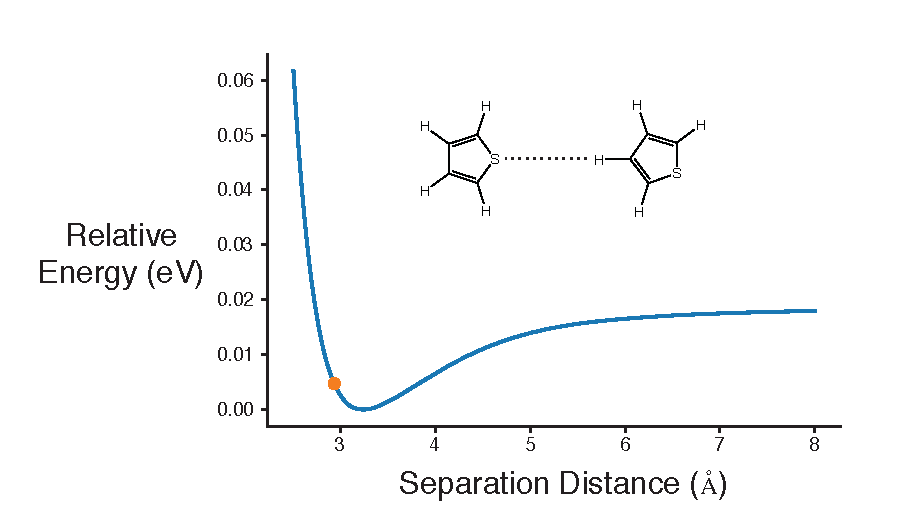
\includegraphics{figures/append_aroma/ts_t_t_copy.pdf}
    \caption{A potential energy scan of the interatomic separation distance between a hydrogen and a sulfur atom on thiophene molecules. The orange dot represents the relaxed H $\cdots$ S distance on a trans (180\textdegree) BT molecule. This indicates that the H $\cdots$ S through-space interaction is marginally repulsive in trans BT. It is noteworthy that the repulsive energy is small compared to the torsional barrier present at 180\textdegree \ in BT (a factor of $\sim$2.5), which in combination with the NCI analysis below demonstrate the minor role of sterics in determining planarity.}
    \label{fig:ts_t_t}
\end{figure}
\clearpage

\subsection{\texorpdfstring{H $\cdots$ S}{HSN} Noncovalent Interaction Analysis}
\begin{figure}[hbt!]
    \centering
    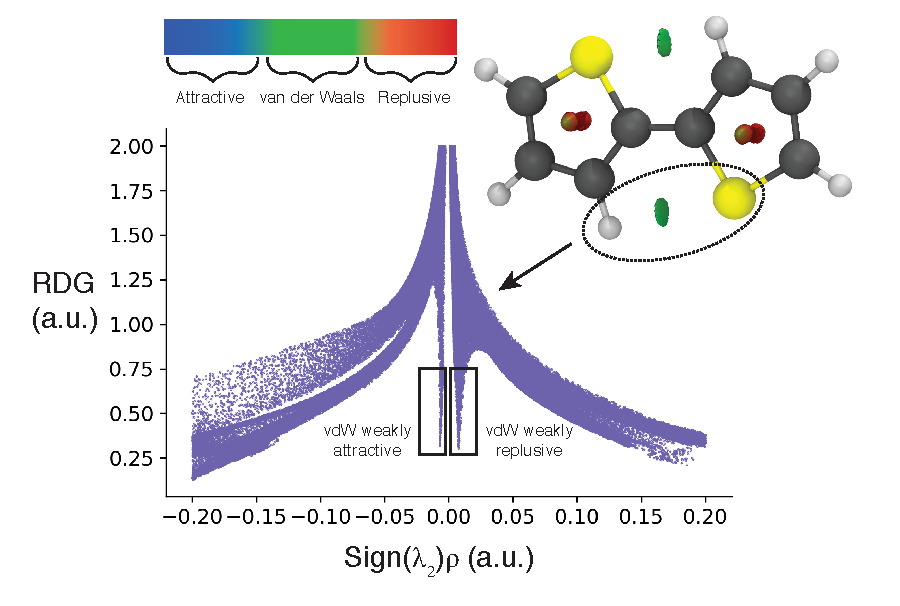
\includegraphics{figures/append_aroma/pt_nci_copy.pdf}
    \caption{The NCI analysis of BT including an NCI isosurface (right) and an s$(\rho$) plot (center), which displays the reduced density gradient (RDG) as a function of the sign of the electron-density Hessian matrix's second eiganvalue (sign$(\lambda_{2})$) times the electron-density ($\rho$). The isosurface plot on right shows a van der Waals interaction between H $\cdots$ S. The color gradient at the top gives a rough physical description of the color scheme used for the isosurface. When only the localized region around H $\cdots$ S is considered, by employing a radius cutoff, the s$(\rho$) plot is inconclusive exhibiting both weakly repulsive and weakly attractive interactions.}
    \label{fig:pt_nci}
\end{figure}
\clearpage

\subsection{\texorpdfstring{F $\cdots$ S}{FS}}
\begin{figure}[hbt!]
    \centering
    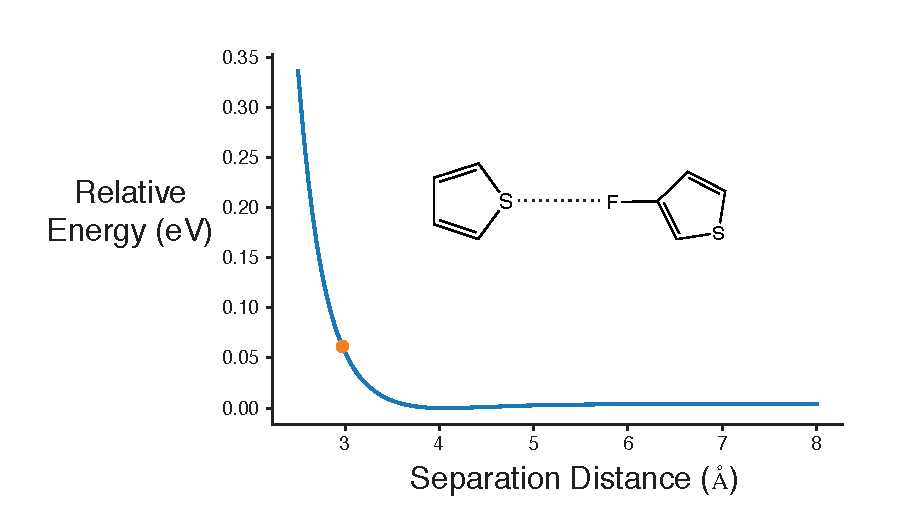
\includegraphics{figures/append_aroma/ts_t_t_f1_copy.pdf}
    \caption{A potential energy scan of the interatomic separation distance between a fluoride and a sulfur atom on a fluorinated thiophene and a thiophene molecule. The orange dot represents the relaxed F $\cdots$ S distance on a trans (180\textdegree) 3F-BT molecule. This indicates that the F $\cdots$ S through-space interaction is repulsive in trans 3F-BT.}
    \label{fig:ts_t_t_f1}
\end{figure}

\begin{figure}[hbt!]
    \centering
    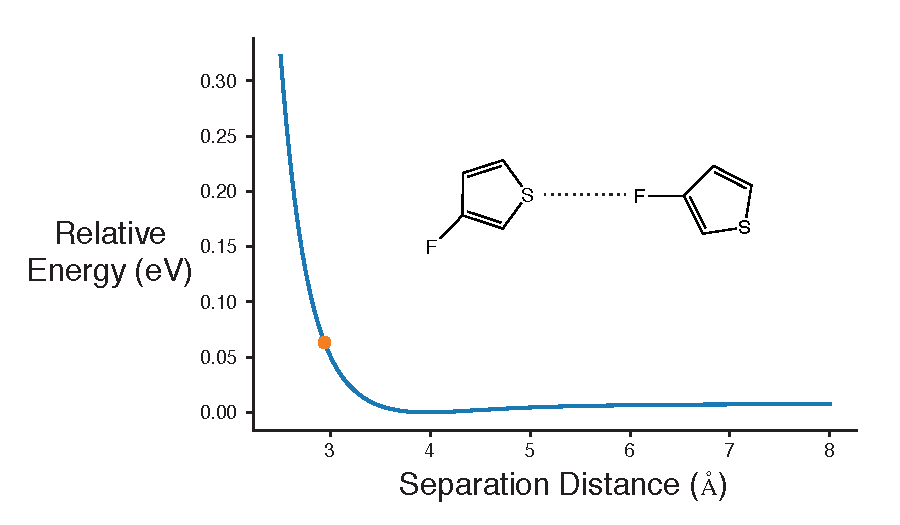
\includegraphics{figures/append_aroma/ts_2t_f1_copy.pdf}
    \caption{A potential energy scan of the interatomic separation distance between a fluoride and a sulfur atom on a fluorinated thiophene molecules. The orange dot represents the relaxed F $\cdots$ S distance on a trans (180\textdegree) F2-BT molecule. This indicates that the F $\cdots$ S through-space interaction is repulsive in trans F2-BT.}
    \label{fig:ts_2t_f1}
\end{figure}
\clearpage

\subsection{\texorpdfstring{F $\cdots$ S}{FSN} Noncovalent Interaction Analysis}
\begin{figure}[hbt!]
    \centering
    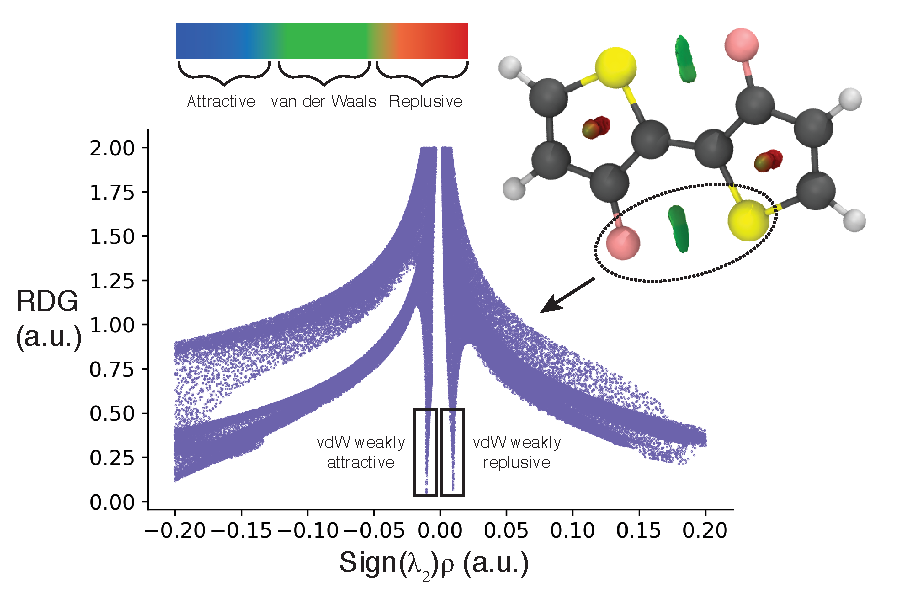
\includegraphics{figures/append_aroma/pt_f2_nciplot_copy.pdf}
    \caption{The NCI analysis of F2-BT including an NCI isosurface (right) and an s$(\rho$) plot (center), which displays the reduced density gradient (RDG) as a function of the sign of the electron-density Hessian matrix's second eiganvalue (sign$(\lambda_{2})$) times the electron-density ($\rho$). The isosurface plot on right shows a van der Waals interaction between H $\cdots$ S. The color gradient at the top gives a rough physical description of the color scheme used for the isosurface. When only the localized region around H $\cdots$ S is considered, by employing a radius cutoff, the s$(\rho$) plot is inconclusive exhibiting both weakly repulsive and weakly attractive interactions.}
    \label{fig:pt_f2_nci}
\end{figure}
\clearpage

\subsection{\texorpdfstring{O $\cdots$ S}{OS}}
\begin{figure}[hbt!]
    \centering
    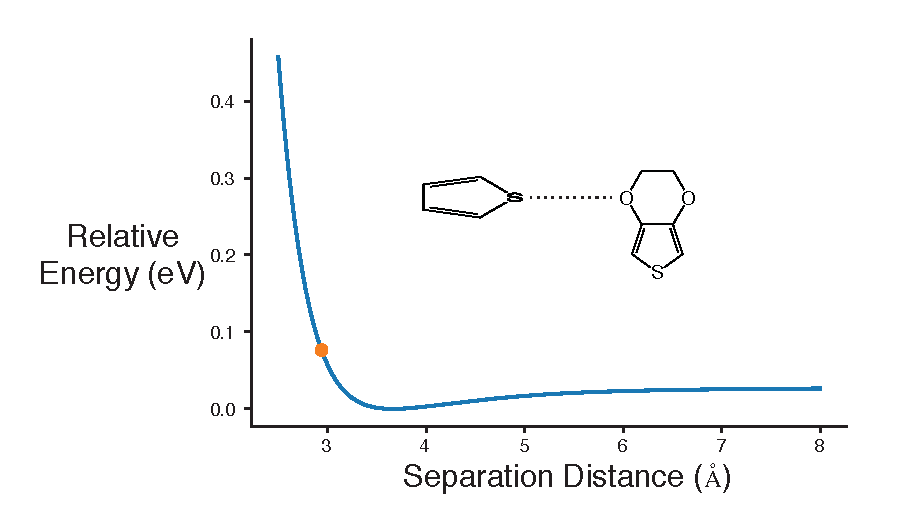
\includegraphics{figures/append_aroma/ts_t_edot_copy.pdf}
    \caption{A potential energy scan of the interatomic separation distance between a oxygen and a sulfur atom on an EDOT and thiophene molecule respectively. The thiophene molecule has been rotated such the ring is perpendicular to the EDOT ring, this is done to minimize secondary H $\cdots$ S interactions. The orange dot represents the relaxed O $\cdots$ S distance on a trans (180\textdegree) BEDOT molecule. This indicates that the O $\cdots$ S through-space interaction is repulsive in trans BEDOT.}
    \label{fig:ts_t_edot}
\end{figure}
\clearpage

\subsection{\texorpdfstring{O $\cdots$ S}{OSN} Noncovalent Interaction Analysis}
\begin{figure}[hbt!]
    \centering
    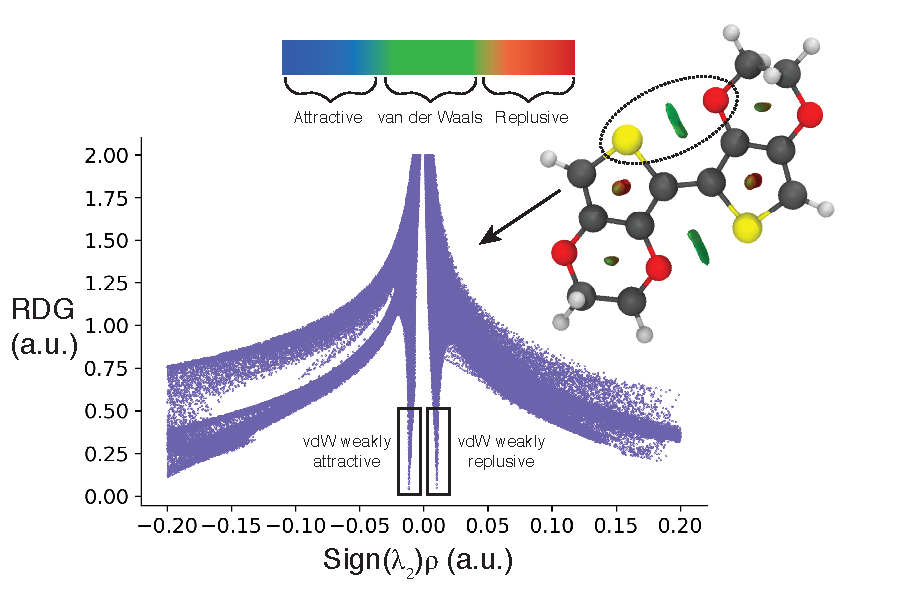
\includegraphics{figures/append_aroma/pedot_nciplot_copy.pdf}
    \caption{The NCI analysis of BEDOT including an NCI isosurface (right) and an s$(\rho$) plot (center), which displays the reduced density gradient (RDG) as a function of the sign of the electron-density Hessian matrix's second eiganvalue (sign$(\lambda_{2})$) times the electron-density ($\rho$). The isosurface plot on right shows a van der Waals interaction between H $\cdots$ S. The color gradient at the top gives a rough physical description of the color scheme used for the isosurface. When only the localized region around H $\cdots$ S is considered, by employing a radius cutoff, the s$(\rho$) plot is inconclusive exhibiting both weakly repulsive and weakly attractive interactions.}
    \label{fig:pedot_nci}
\end{figure}
\clearpage
